
 \documentclass{article}
 \usepackage{amsmath}
 \usepackage{graphicx}
 \usepackage{float}
 \usepackage{listings}
 \lstset{language=Octave,basicstyle=\ttfamily,commentstyle=\ttfamily}
 \title{\textsf{OctLatex}: Embedding \textsf{Octave} Results in \LaTeX\ Documents\\ {\small version 2022.02.05}}
 \author{Athanasios Kehagias\\kehagiat@ece.auth.gr}
 \setlength{\textwidth}{6.75in}
 \setlength{\textheight}{9.00in}
 \setlength{\oddsidemargin}{0 in}
 \setlength{\topmargin}{0 in}
 \begin{document}
 \maketitle
 \section{Introduction}
 \texttt{OctLatex.m} is a \emph{very simple} script intended to enable the user to \emph{programmatically} 
 include the results of \textsf{Octave} computations in \LaTeX\  documents;
 the focus is on \emph{symbolic} computations but numerics and figures can also be used. 
 Hence it is similar in purpose to the various ``sweave'' packages that exist for \textsf{Matlab}, 
 \textsf{SageMath}, \textsf{R}, \textsf{Python} etc. But the emphasis of \textsf{OctLatex} is on \emph{simplicity}.
 \footnote{Further discussion of this point appears in the Postscript.}

 \section{Installation}
 Simply unzip the file \texttt{OctLatex.zip} into some folder. You must have installed \textsf{Octave}, 
 the  \textsf{Octave Symbolic Math Package} and a \TeX\  distribution. 
 I have tested \textsf{OctLatex} with \textsf{Octave6.4.0} and \textsf{TeX Live 2019}.
 It works on \textsf{Windows 7, 10, 11}; since it only depends on \textsf{Octave} and \LaTeX\,
 it should also work on the \textsf{Linux} and \textsf{Apple} operating systems
 (but I have not tested this).
 
 \section{QuickStart}
 In the \textsf{Octave} environment, run the script \texttt{OctLatex.m}. 
 You will get the files \texttt{OctLatex.tex} and \texttt{OctLatex.pdf} (this document).
 Open \texttt{OctLatex.m} to see the code which produces the results of this document
 (the contents of \texttt{OctLatex.m} will be explained in a later section).
 
 \section{Usage}
 The \textsf{OctLatex} workflow is as follows. 
 \begin{enumerate}
 \item Write a \emph{single} \textsf{Octave} script, e.g., \texttt{foo.m}, 
 which contains both \textsf{Octave} commands and \LaTeX\  code (embedded as comments);
 the \LaTeX\  code can include the control words \texttt{latex (a)} and \texttt{num2str(b)} 
 where \texttt{a} and \texttt{b} are \textsf{Octave} variables (details will be given in the following sections).    
 \item The file \texttt{foo.m} must be created in the same folder which contains \texttt{OctLatex.m}.
 \item Change the second line of \texttt{OctLatex.m} from \texttt{fn='OctLatexDoc'} to \texttt{fn='foo'}.
 \item Run \texttt{OctLatex.m} (i.e., type \texttt{OctLatex} in the \textsf{Octave} command line).
 \item When execution of \texttt{OctLatex.m} is completed you have the following files.
 \begin{enumerate}  
 \item \texttt{foo.tex}: your \LaTeX\  code with \textsf{Octave} results having replaced
 the \texttt{latex (a)} and \texttt{num2str(b)} control words.
 \item \texttt{foo.pdf}: the output of \texttt{foo.tex} as compiled by \textsf{pdflatex}.
 \end{enumerate}
 \end{enumerate}
 
 \noindent To use \textsf{OctLatex} follow the above  workflow.
 The rules for writing \textsf{OctLatex} files are as follows.
 \begin{enumerate}
 \item Each line contains either \emph{only} \textsf{Octave} code  or \emph{only} \LaTeX\ code. 
 \item \textsf{Octave} code is written as usual.
 \item \LaTeX\ code is also written as usual with the following exceptions. 
 \begin{enumerate}
 \item Every line of \LaTeX\ code is preceded by the characters \texttt{\%\%} 
 (so, as far as \textsf{Octave} is concerned, these
 are comment lines).
 \item You can use the additional control word \texttt{latex (\;)} (\textbf{without} being preceded by a backslash!). 
 Every occurrence of \texttt{a} in the \LaTeX\  part of your code will be replaced 
 by the \LaTeX\  expression for \texttt{a},
 where it is assumed that \texttt{a} has been declared (in the \textsf{Octave} part of your code) as a symbolic variable.
 \item You can use the additional control word \texttt{num2str(\;)} (\textbf{without} being preceded by a backslash!).
 Every occurrence of \texttt{num2str(a)} in the \LaTeX\ part of your code will 
 be replaced by the \texttt{num2str}  expression for  \texttt{a},
 where it is assumed that \texttt{a} has been declared / computed (in the \textsf{Octave} part of your code) 
 as a $1\times 1$ double variable. 

 \medskip 
 
 \noindent\textbf{Nota Bene}:
 This means that you can only use \texttt{num2str (\;)} to render \emph{scalar} doubles. If you want 
 to render a double matrix \texttt{A},
 you must define a symbolic variable \texttt{Z} by \texttt{B=sym(A)} and then use \texttt{latex(Z)}. This works well when 
 the entries of \texttt{A} are integers or simple fractions; but if \texttt{A} has entries with many decimals,
 \texttt{Z}  will be represented by fractions with large integer numerators and denominators. So this 
 is an issue which I hope to fix at a later version of \textsf{OctLatex}.

 \end{enumerate}  
 \end{enumerate}  

 \section{Some Examples and Explanations}
 Let us now look at some parts of \texttt{OctLatexDoc.m}.
 \begin{enumerate}
 \item The file starts with the lines 
 \begin{lstlisting}
 %% \documentclass{article}
 %% \usepackage{amsmath}
 %% \usepackage{graphicx}
 \end{lstlisting}
 and continues like this with typical \LaTeX\ preamble commands. Note that, since these are 
 \LaTeX\ commands, they are preceded by \texttt{\%\%}.
 \item After a while we have  
 \begin{lstlisting}
 %% \begin{document}
 %% \maketitle
 %% \section{Introduction}
 %% \texttt{OctLatex.m} is a \emph{very simple} script intended to 
 %% implement \emph{literate programming} in \textsf{Octave}. 
 \end{lstlisting}
 and so on, where we write our \LaTeX\ content as usual, but always using the \texttt{\%\%} line prefix.
 \item Things get more interesting when we introduce symbolic computations. So for example the code 
 \begin{lstlisting}
 syms x
 syms f(x)
 f(x)=x*exp(x);
 F(x)=int(f,x);
 %% Let us write the integral of \(f(x)=latex (f)\), 
 %% i.e., \( \int latex (f) dx = latex (F)\).
 \end{lstlisting}
 produces the following results.
 
 \qquad Let us write the integral of \(f(x)=x e^{x}\), i.e., \( \int x e^{x} dx = \left(x - 1\right) e^{x}\).

 Similarly,  the code
 \begin{lstlisting}
 syms n
 syms g(n)
 g(n)=1/n^2;
 G=symsum(g,n,1,inf);
 G0=double(G);
 %% Let us write the sum of \(g(n)=latex (g)\), i.e., 
 %% \(\sum_{n=1}^\infty latex (g)  = latex (G)\). 
 %% This evaluates to \( latex (G) = num2str (G0)\). 
 \end{lstlisting}
 produces the following results.

 \qquad Let us write the sum of \(g(n)=\frac{1}{n^{2}}\), i.e., 
 \(\sum_{n=1}^\infty \frac{1}{n^{2}}  = \frac{\pi^{2}}{6}\). 
 This evaluates to \( \frac{\pi^{2}}{6} = 1.6449\).
 \item We can also include plots. For example,  the following code
 \begin{lstlisting}
 fh=figure(1); plot([0:0.1:4*pi],sin(2*[0:0.1:4*pi])); axis([0 4*pi -1.1 1.1]);
 print(fh,"FIG001",'-dpdflatexstandalone','-r600');
 %% \begin{figure}[H]
 %% \centering
 %% 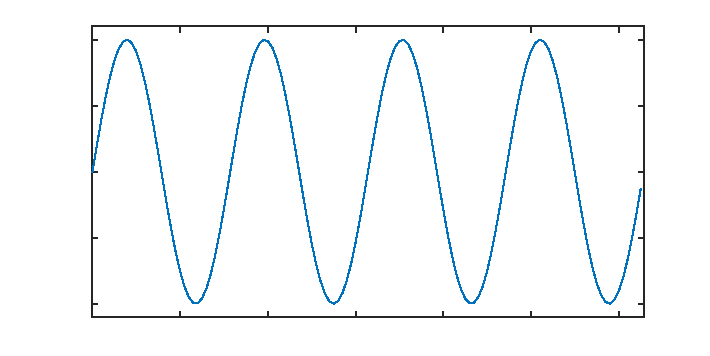
\includegraphics[scale=0.75]{FIG001-inc}
 %% \caption{A plot of \(f(x)=\sin(2*x)\).}
 %% \end{figure}
 \end{lstlisting}
 produces the plot:
 \begin{figure}[H]
 \centering
 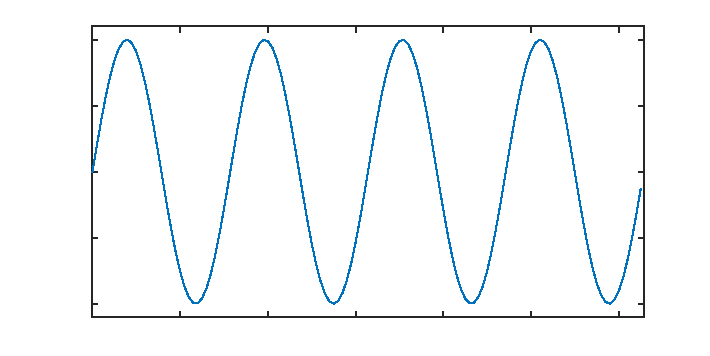
\includegraphics[scale=0.75]{FIG001-inc}
 \caption{A plot of \(f(x)=\sin(2*x)\).}
 \end{figure}
 The idea is the following. The first line of the above fragment 
 generates a ``regular'' \textsf{Octave} plot and the second line prints it to file \texttt{FIG001.pdf}.
 The final five lines are regular \LaTeX\ code which ``graphics -includes'' the previously produced file.
 
 \item Let us now present  some additional symbolic results; to see the code which
 generates the following lines open \textsf{OctLatexDoc.m} and look at around lines 180-260.
 \begin{enumerate}
 \item The Hessian of \(f(x,y,z)=2 x^{2} z + x y^{2}\) is
 \[
 H=\left[\begin{matrix}4 z & 2 y & 4 x\\2 y & 2 x & 0\\4 x & 0 & 0\end{matrix}\right]
 \]
 \item The Jacobian of \(f(x,y,z)=2 x^{2} z + x y^{2}\) is
 \[
 J=\left[\begin{matrix}4 x z + y^{2} & 2 x y & 2 x^{2}\end{matrix}\right]
 \]
 \item An algebraic expansion
 \[
 \left(x - y\right) \left(x^{2} + x y + y^{2}\right)=x^{3} - y^{3}
 \]
 \item Let us solve the equation \(x^{2} + x + 1 = 0\). It has the roots
 \[
 r_1=- \frac{1}{2} - \frac{\sqrt{3} i}{2}, \qquad r_2=- \frac{1}{2} + \frac{\sqrt{3} i}{2}. 
 \]
 \item Let us solve the differential equation \(\frac{d}{d t} u{\left(t \right)} = t u{\left(t \right)}\). It has the family of solutions
 \[
 u(t)=u{\left(t \right)} = C_{1} e^{\frac{t^{2}}{2}}. 
 \]
 \item We can write a matrix and compute its inverse
 \[
 A=\left[\begin{matrix}1 & 2\\3 & 4\end{matrix}\right] \qquad \text{and} \qquad A^{-1}=\left[\begin{matrix}-2 & 1\\\frac{3}{2} & - \frac{1}{2}\end{matrix}\right]
 \]
 \item The same thing with a matrix which includes symbols
 \[
 B=\left[\begin{matrix}a & b\\c & d\end{matrix}\right] \qquad \text{and} \qquad B^{-1}=\left[\begin{matrix}\frac{d}{a d - b c} & - \frac{b}{a d - b c}\\- \frac{c}{a d - b c} & \frac{a}{a d - b c}\end{matrix}\right]
 \]
 \item Here is a Laplace transform.
 \[
 {\cal L}(a \cos{\left(t w_{0} \right)})=\frac{a s}{s^{2} + w_{0}^{2}}.
 \]
 \item Here is a 3d  plot (look up the corresponding code in \texttt{OctLatexDoc.m}).
 \begin{figure}[H]
 \centering
 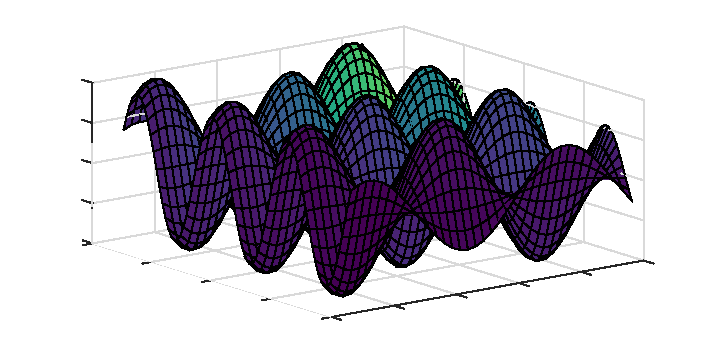
\includegraphics[scale=0.85]{FIG002-inc}
 \caption{A plot of \(f(x,y)=\sin(x)\cos(y)\).}
 \end{figure}
 \end{enumerate}
 \bigskip
 
 \end{enumerate}  

 \section{Postscript}
 My motivation for writing \textsf{OctLaTex} was the need for a simple system to create problem sets and exams 
 (and answers!) for my math classes. I have been using several computer algebra systems: 
 the symbolic math toolboxes of \textsf{Matlab} and \textsf{Octave}, \textsf{Maple}, \textsf{SageMath}, \textsf{SymPy} and so on.
 Not wanting to reinvent the wheel I looked at what was available. I started with \textsf{SageTex}; alas, I was
 never able to properly install and run it. I tried several additional packages and I found each one either 
 too confusing to set up, or not providing the functionalities I wanted, or both.
 
 Consequently I decided to write my own package. I am a simple guy and \textsf{OctLaTex} is a simple hack. 
 I am certain that any sufficiently interested serious programmer can produce a much better version
 and I will be very happy if someone does. 
 In the meantime, \textsf{OctLaTex} works  right out of the box and does what I want it to do: 
 programmatically incorporate symbolic and numeric \textsf{Octave} results into my \LaTeX\  documents. 
 
 In conclusion, there are a few improvements / extensions on which I hope to work in the future. I list them 
 in order of decreasing priority. 
 \begin{enumerate}
 \item In the current implementation, variable names cannot be ``reused''. If a variable \texttt{a} appears several times
 in the \LaTeX\ commands, it will always be replaced by its last computed value. I would like to be able
 to replace each occurrence of \texttt{a} with its value as computed just before this appearance.
 \item Double matrices should be handled better.
 \end{enumerate}
 \noindent Finally, let me mention that I am also working on \textsf{MatLatex} and \textsf{MapleLatex} which are 
 \textsf{Matlab} and \textsf{Maple} versions of the \textsf{OctLaTex} idea.

 \end{document}  